\section{Generating initial structures}
\textbf{Two different methods are used to distribute particles and provide them with initial velocities. One generates completely isotropic structures, the other tunes the degree of velocity anisotropy by a free parameter.} \\ 

\subsection{Eddingtons inversion method}
\textbf{Eddingtons inversion method is used to construct isotropic spherical models.} \\ 

If we know the density profile of a spherical structure with potential $\Phi(r)$ then a unique DF depending on the phase-space coordinates only through the Hamiltonian H(x,v) can be found. As it depends only on the energy this DF f($\mathcal{E}$) is ergodic and has $\beta = 0$ everywhere by definition. Introducing the relative energy 
\begin{equation} 
\mathcal{E} \equiv -\Phi+\Phi_0
\end{equation}
and relative potential 
\begin{equation} 
\Psi \equiv -H+\Phi_0 = \Psi - \frac{1}{2}v^2
\end{equation}
The PDF $\nu(r)$ is the integral of f over all velocities.  
\begin{equation} 
f(\mathcal{E}) = 4\pi \int \! v^2 f(\Psi - \frac{1}{2}v^2) \, \mathrm{d}v =
4\pi \int_{0}^{\Psi} \! f(\mathcal{E}) \sqrt{2(\Psi - \mathcal{E})} \, \mathrm{d}\mathcal{E} =
4\pi \cdot \sqrt{2} \int_{0}^{\Psi} \! f(\mathcal{E}) \sqrt{\Psi - \mathcal{E}} \, \mathrm{d}\mathcal{E}
\end{equation}
Transforming $\nu(r) \rightarrow \nu(\Psi)$ and rearranging (also using $4 \sqrt{2} = 2 \sqrt{8}$),
\begin{equation} 
\frac{1}{\sqrt{8}\pi}\nu(\Psi) = 2\int_{0}^{\Psi} \! f(\mathcal{E}) \sqrt{\Psi - \mathcal{E}} \, \mathrm{d}\mathcal{E}
\end{equation}
Differentiating the above equation wrt $\Psi$ and solving the following Abel integral equation we obtain Eddington's formula which gives us the corresponding distribution function,
\begin{equation} 
f(\mathcal{E}) = \frac{1}{\sqrt{8}\pi^2}\frac{\mathrm{d}}{\mathrm{d}\mathcal{E}}
\int_{0}^{\mathcal{E}} \! \frac{d \Psi}{\sqrt{\mathcal{E}-\Psi}} \, \frac{\mathrm{d}\nu}{\mathrm{d}\Psi} 
\end{equation}
To see this derivation in more details, see [3].
A C-code made publicly available by Martin Sparre is used for this purpose [1]. It takes a density model as argument and uses it to distribute particles and provide them with initial velocities.
\begin{figure}[!htbp]
\centering
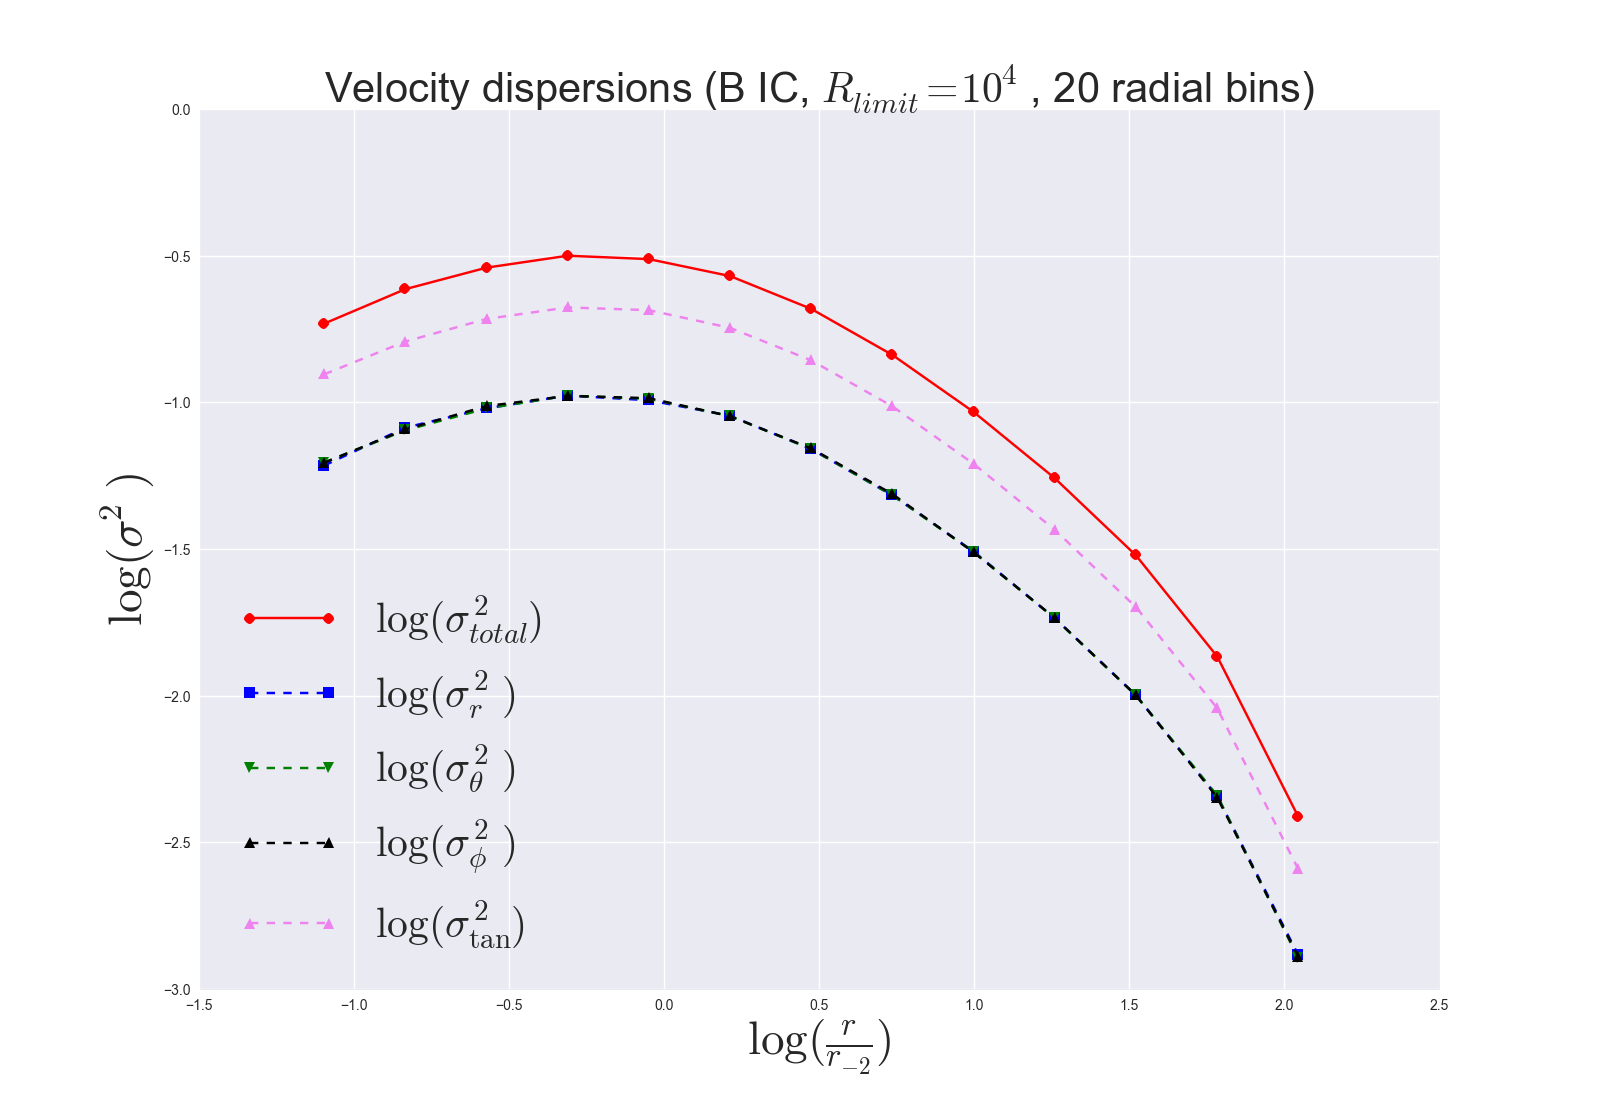
\includegraphics[width=1.0\linewidth]{img/B_IC_sigma_r_2.png}
\caption{$\log (\sigma^2)$ vs. $\log (\frac{r}{r_{-2}})$ for IC of structure B. 20 radial bins is used and the structure is cut off at radius $R_{limit} = 10^4$ in arbitrary units of radius. Notice how each of the dispersions $\sigma_r^2$, $\sigma_{\theta}^2$ and $\sigma_{\phi}^2$ contributes equally to the total velocity dispersion. This is due to the fact that the IC of structure B is completely isotropic (as is the case for any Eddington profile) and therefore $\sigma_r^2 = \sigma_{\theta}^2 = \sigma_{\phi}^2$. This is true throughout all radii of the structure. The pink curve shows the tangential part, $\sigma_{tan}^2 = \sigma_{\theta}^2 + \sigma_{\phi}^2$.}
\label{fig:test}
\end{figure}

\begin{figure}[!htbp]
\centering
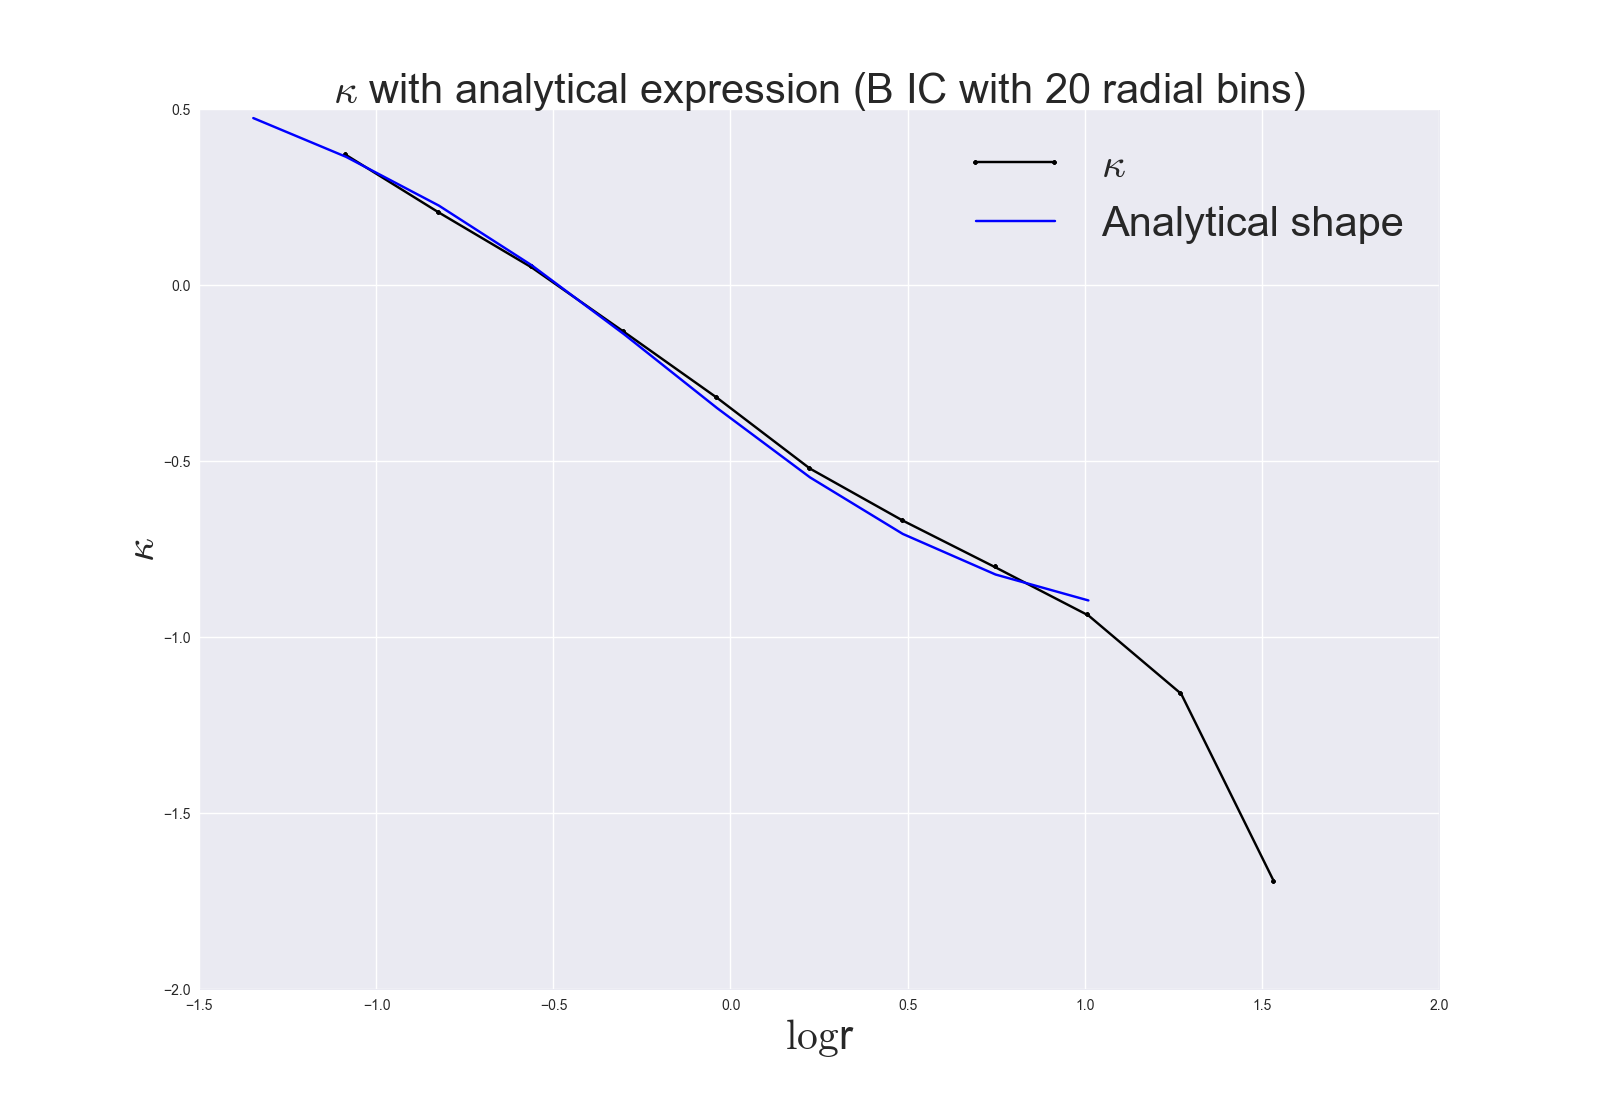
\includegraphics[width=1.0\linewidth]{img/B_IC_kappa_logr_fit.png}
\caption{$\kappa$ for IC of stable structure B shown together with the analytical expression. 20 radial bins is used. This provides a welcome consistency check of the C-codes used from [1] and [2]. The analytical expression is seen to be in good agreement with the structure generated by means of these codes. The analytical expression is truncated around $\log r = 1$ as the two curves starts to depart from each other here. This could be due to different reasons, e.g. the initial value chosen numerically when solving the differential equation arising from the Jeans equation when isolating $\sigma_r^2$ might be needed at higher accuracy or perhaps outer parts of the IC generated using Eddingtons method departs slightly from equilibrium due to the large distances between particles here. The majority of the IC is seen to be in good agreement though.}
\label{fig:test}
\end{figure}

\begin{figure}[!htbp]
\centering
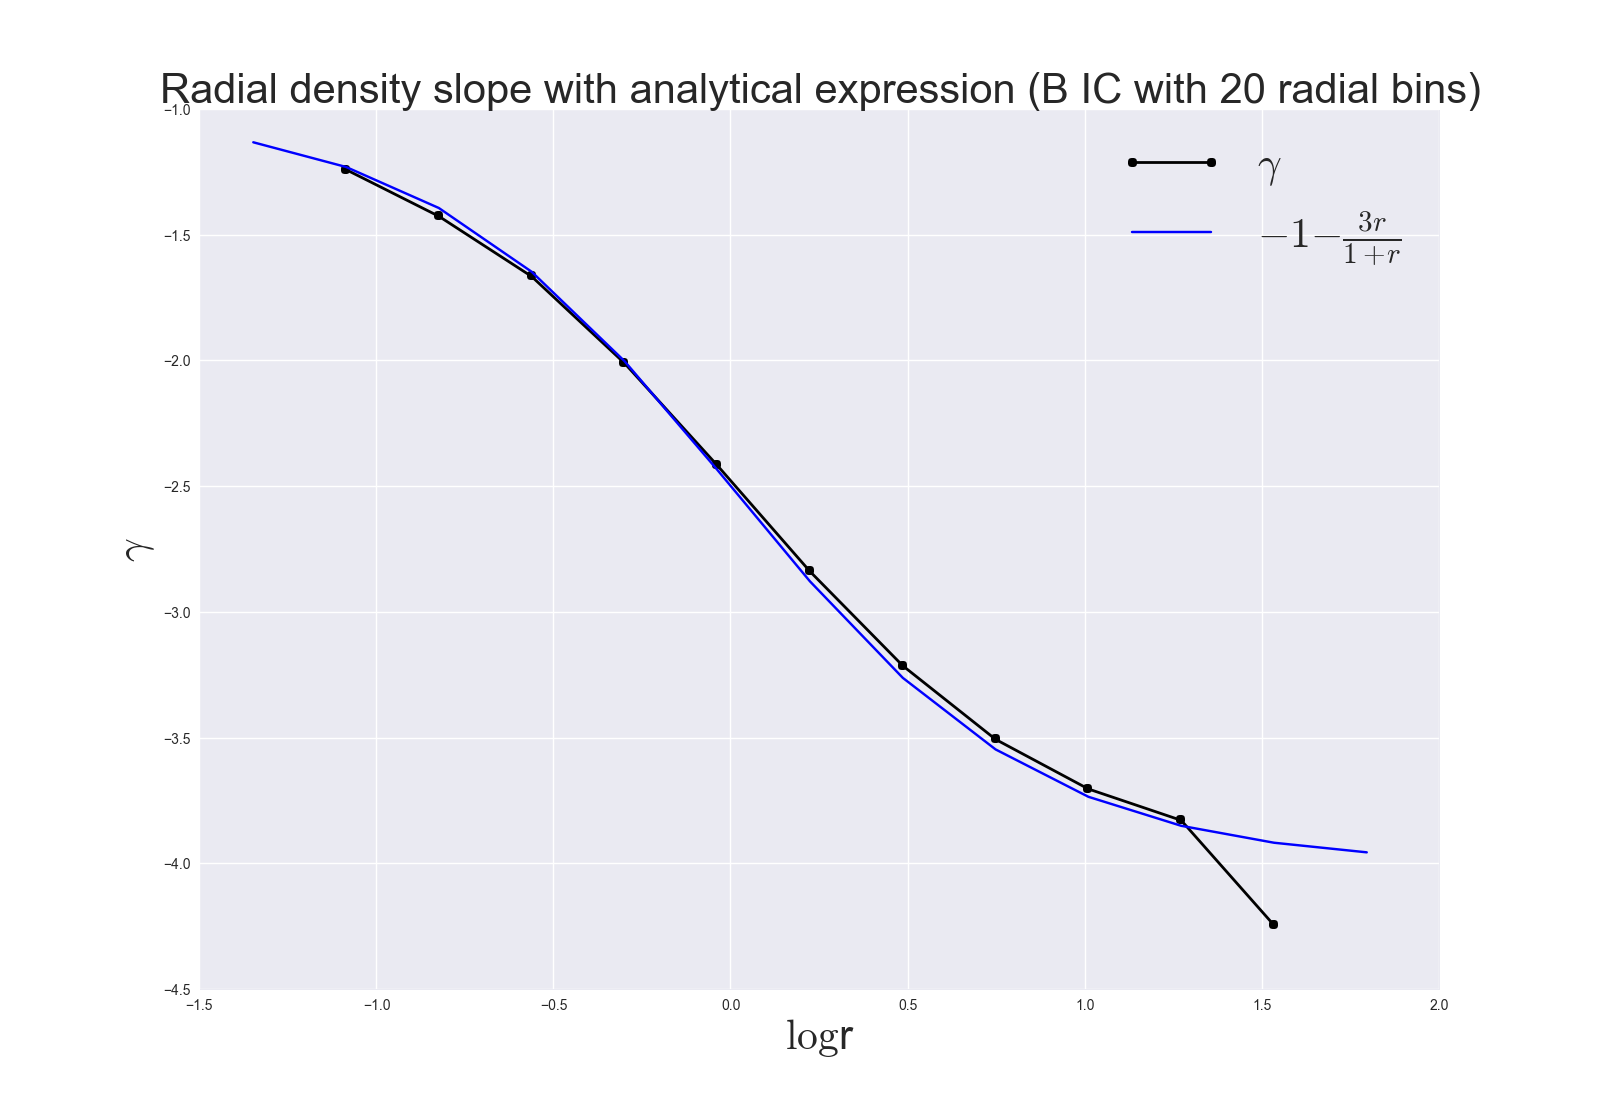
\includegraphics[width=1.0\linewidth]{img/B_IC_gamma_logr_fit.png}
\caption{$\gamma$ for IC of structure B shown together with the analytical expression $\gamma = -1-\frac{3r}{1+r}$. 20 radial bins is used. This provides a welcome consistency check of the C-codes used from [1] and [2]. The analytical expression is seen to be in good agreement with the structure generated by means of these codes.}
\label{fig:test}
\end{figure}

Checks for the validity of the Eddington profiles and the Osipkov-Merritt models (see next section) generated from the C-codes [1] and [2] is provided here graphically by means of over-plotting the Jeans parameter profiles and their corresponding analytical expressions. The results from the C-codes and the analysis codes developed for this work are thus seen to be in good agreement (see figure 4-6).

\centerline{\textbf{Analytical expression of $\gamma$:}}
For a Hernquist density model with scale radius $r_s = 1$,
\begin{equation} 
\rho_{HQ}(r) = \frac{\rho_0}{r(1+r)^3}  
\end{equation}
The natural logarithm can be applied to both sides,
\begin{equation} 
ln(\rho) = ln \Bigg[ \frac{\rho_0}{r(1+r)^3} \Bigg] = ln(\rho_0) - ln(r(1+r)^3)
\end{equation}
Setting $\rho_0 = 1$,
\begin{equation} 
ln(\rho) = - ln(r(1+r)^3) = - ln(r) -3ln(1+r)
\end{equation}
$\gamma$ is defined as 
\begin{equation}
\gamma \equiv \frac{d\ln\rho}{d\ln r} = r\cdot \frac{d\ln\rho}{dr} = 
r\cdot \Bigg( -\frac{1}{r}-3\cdot \frac{1}{1+r} \Bigg) =
-1-\frac{3r}{1+r}
\end{equation}
which is thus the analytical expression.
This can be seen in figure 5 to agree very well with the IC of Eddington structure B.


\centerline{\textbf{Analytical expression of $\kappa$:}}
This Jeans parameter can be derived analytically by solving the differential equation arising when $\kappa = -\frac{d\ln\sigma_r^2}{d\ln r} $ is isolated from the Jeans Equation assuming e.g. a Hernquist density profile. As we are considering isotropic models here, $\beta = 0$ and J.E. reads

\begin{equation}
M(r)= -\frac{r \sigma_r^2}{G} \big[\gamma +\kappa] 
\end{equation}
rearranging,
\begin{equation}
-\frac{GM}{r} = \sigma_r^2 \big[\gamma +\kappa] 
\end{equation}
isolating $\kappa$,
\begin{equation}
\kappa = -\frac{GM}{r \sigma_r^2} - \gamma
\end{equation}
using the definition,
\begin{equation}
\kappa = \frac{d\ln\sigma_r^2}{d\ln r} = \frac{r}{\sigma_r^2}\cdot \frac{d \sigma_r^2}{dr}
\end{equation}
equating the two expressions for $\kappa$,
\begin{equation}
\frac{r}{\sigma_r^2}\cdot \frac{d \sigma_r^2}{dr} = -\frac{GM}{r \sigma_r^2} - \gamma
\end{equation}
multiplying both sides by $\frac{\sigma_r^2}{r}$,
\begin{equation}
\frac{d \sigma_r^2}{dr} = -\frac{GM}{r^2} - \frac{\gamma \sigma_r^2}{r} 
\end{equation}
which can then be solved for $\sigma_r^2$ when inserting the analytical expression for $\gamma$ found above and when using the initial value of \[ \lim_{r \to \infty} \sigma_r^2 = 0 \] (which can be approximated numerically as e.g. (r,$\sigma_r^2$) = ($10^5$,$10^{-5}$) to solve computationally).
After $\sigma_r^2$ is found, $\kappa$ is determined by the definition $\kappa = -\frac{d\ln\sigma_r^2}{d\ln r} $, in a similar fashion as the one utilized for deriving $\gamma$ above.
The resulting expression is very long so it is omitted here but can be seen in figure 4 to agree very well with the IC of Eddington structure B (to see the full analytical expression go to the link for my analysis codes given in the conclusion to this project).

\subsection{Osipkov-Merritt models}
\textbf{This method generalizes Eddington's formula. Whereas Eddington's formula simply creates isotropic structures, OM models can have anisotropy as well.} \\ 

Spherical stellar systems such as galaxies and star clusters as well as dark matter halos can be represented mathematically by OM models. Ansatz: The DF depends on another function, Q: $f(Q) = f(\mathcal{E} - \frac{L^2}{2r_a^2})$ This creates DF's in phase-space which belong to specified density profiles; e.g. of a DM halo, in a predefined gravitational potential. The degree of velocity anisotropy is adjusted by the anisotropy radius $r_a$. When the minimum value $r_a=0$ is used, the model will be isotropic and produce the same outcome as Eddington's method. At the other extreme, when $r_a=\infty$, the model will consist of purely radial motions. The OM DF has the form
\begin{equation} 
f(Q) = \frac{1}{\sqrt{8}\pi^2} \Bigg[ \int_{0}^{Q} \! \frac{\mathrm{d} \Psi}{\mathrm{d} \sqrt{Q-\Psi}}
\frac{\mathrm{d}^2 \nu_Q}{\mathrm{d} \Psi^2} + \frac{1}{\sqrt{Q}} \Bigg( \frac{\mathrm{d} \nu_Q}{\mathrm{d} \Psi} \Bigg)_{\Psi=0} \Bigg]
\end{equation}
The anisotropy parameter is given by 
\begin{equation} 
\beta(r) = \frac{1}{1+(\frac{r}{r_a})^2}
\end{equation}
This gives a structure which has $\beta = 0 $ for $r<<r_a$ and radially biased for $r>>r_a$ I am using a C code made publicly available by Martin Sparre [2].
\begin{figure}[!htbp]
\centering
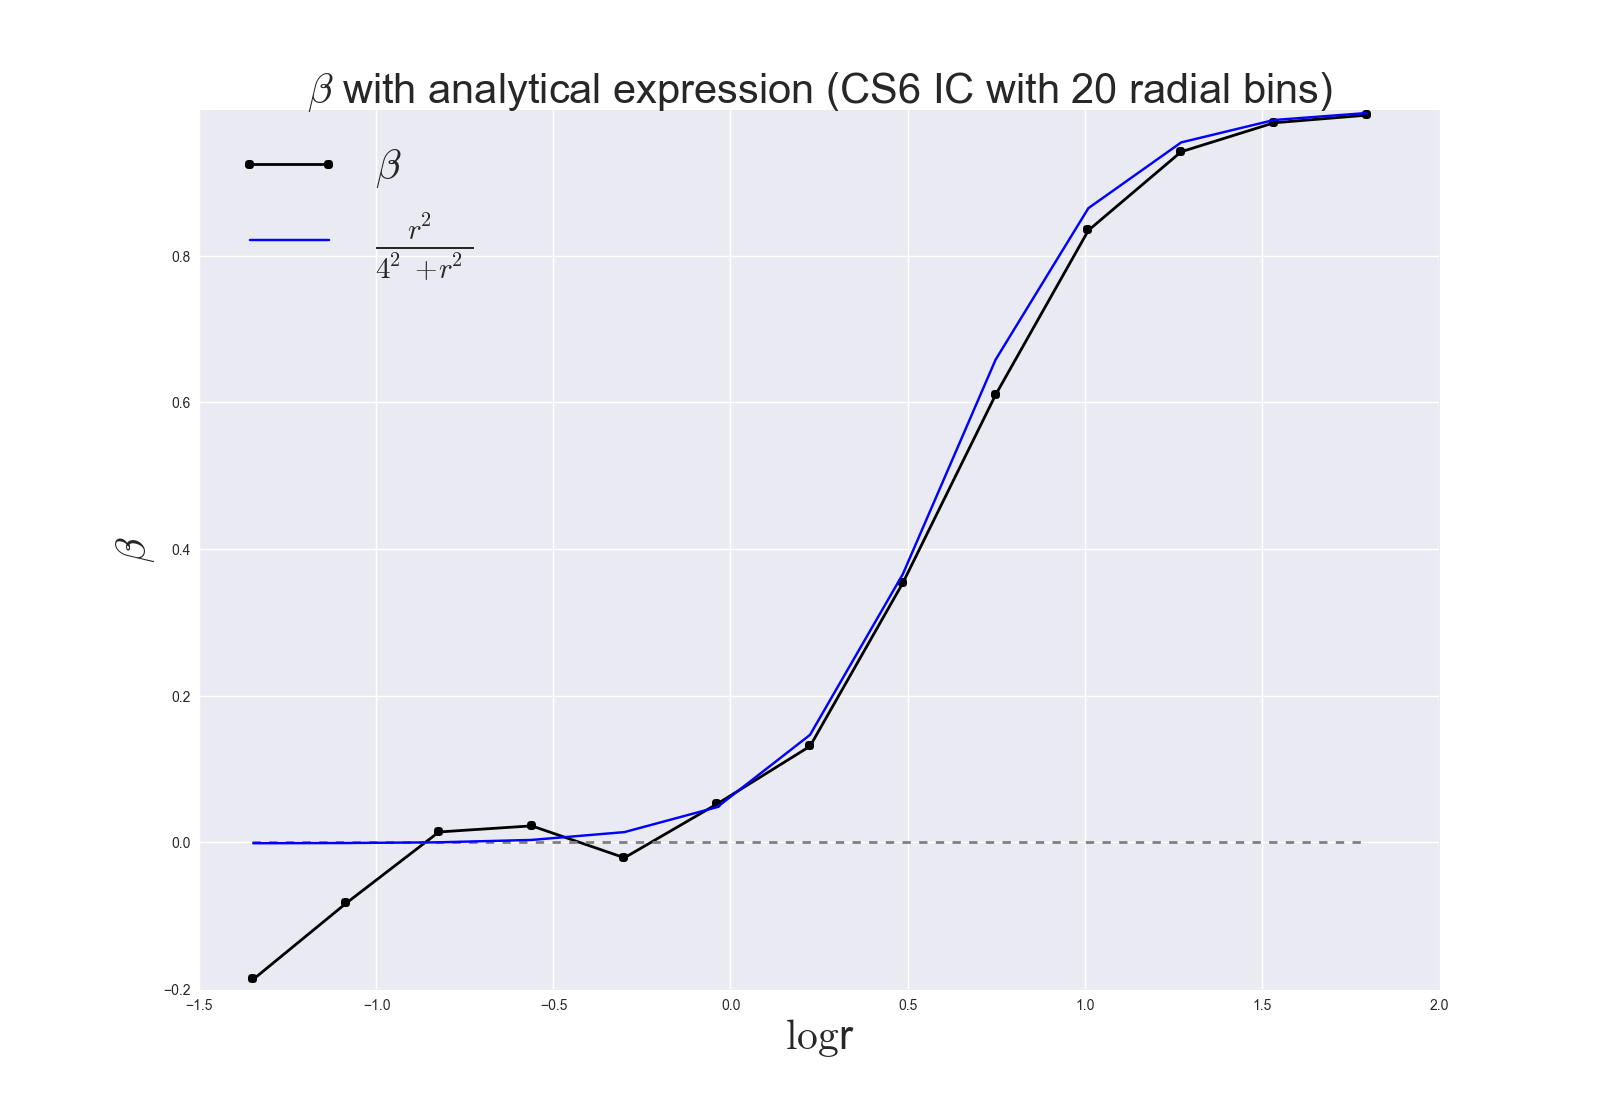
\includegraphics[width=1.0\linewidth]{img/CS6_IC_beta_logr_fit.png}
\caption{$\beta$ for IC of structure CS$\_$6 shown together with the analytical expression $\beta(r)=\frac{r^2}{r_a^2+r^2}$. It is seen that the analytical expression agrees well with the computed velocity anisotropy for the anisotropy radius $r_a = 4.0$, which is the value specified for the IC of the CS$\_$6 structure. 20 radial bins is used.}
\label{fig:test}
\end{figure}

\centerline{\textbf{Analytical expression of $\beta$:}}
The $\beta$ expression for an OM model is simply given by $\beta(r)=\frac{r^2}{r_a^2+r^2}$ so if we choose to set $r_a = 1$, the analytical form becomes just $\beta(r)=\frac{r^2}{1+r^2}$ which can be seen in figure 6 to agree very well with the IC of OM model CS$\_$6.

\subsection{Overview of structures}
\textbf{All structures can be divided into two categories, namely stable or unstable (see tables). Most of them follow Hernquist density profiles (see previous section) but three follow the $(\alpha, \beta) = (0,5)$ density profile. The unstable structures are dealt with in the later section 'Unstable OM models'. ICs have been chosen so that they together span a large volume in the 3D Jeans parameter solution space ($\beta, \gamma, \kappa$). This creates an opportunity to test if they all keep spanning a large volume or flow towards an attractor.} \\ 

Since all HQ structures have a total mass of unity but vary in particle number, the more numerous structures have particles with lower mass. Variations in anisotropy radius are carried out while setting up the different OM models. Gravitational softening is varied so that it decreases by a factor when particle number is increased (see tables). For all simulations, the scale radius $r_s = 1$ is used and $\rho_0 = \frac{1}{2 \pi}$ (which ensures that all HQ structure has a total numerical mass value of 1). The type of simulation each structure is undergoing is indicated by I: 'Instantaneous change in the gravitational potential' and II: 'Energy exchange' (See later sections for description of I and II). 
\begin{table}[!htbp]
\centering
\begin{tabular}{|c|c|c|c|c|c|c|c|c|c|c|c|}
\hline
 &A&B&$CS_1$&$CS_2$&$CS_3$&$CS_4$&$CS_5$&$CS_6$&$DS_1$&$D_2$&E \\ \hline
 N &$10^6$&$10^6$&$10^4$&$10^4$&$10^4$&$10^5$&$10^5$&$10^5$&$10^5$&$10^5$&$10^6$ \\ \hline
 IC&Edd&Edd&OM& OM & OM & OM & OM & OM & OM & Edd & OM                \\ \hline
 $\rho$ & HQ & HQ & HQ & HQ & HQ & HQ & HQ & HQ & (0,5) & (0,5) & HQ  \\ \hline
 $r_a$ & - & - & 1.33 & 1.5 & 2.0 & 1.5 & 2.0 & 4.0 & 2.0 & - & 2.0   \\ \hline
 $\epsilon$&0.1&0.1,0.02&0.1&0.1&0.1&0.04&0.04&0.04&0.04&0.1,0.04&0.02\\ \hline
 SIMS & I & I,II & II & - & - & I,II & I,II & I, II & I,II & I,II & I,II \\ \hline
 $\Delta G$ & 20\% & 5\% & - & - & - & 20\% & 20\% & 20\% & 20\% & 20\% & 20\% \\ \hline
\end{tabular}
\caption {Stable structures. From top to bottom this table states the name of each stable structure, the total number of particles this structure holds (N), the method utilized for setting up the initial conditions (IC's), the type of double-power law model used for creating this structure, for Osipkov-Merritt (OM) models the anisotropy radius is then given. Next follows the value of the gravitational softening, $\epsilon$, the types of simulations the different structures are subjected to (I: G-perturbations or II: Energy exchange), for sim. I the percentage of variation to Newtons gravitational constant is then stated and finally for sim. II the maximum percentage (most particles are subjected to a variation in velocity of size smaller than this percentage since random uniform numbers in the given range dictate the size of each velocity kick, see the later section 'II: Energy exchange' for more details about this sim.) of variation to each particles velocity is stated.}
\end{table}
\begin{table}[!htbp]
\centering
\begin{tabular}{|c|c|c|c|c|c|c|c|}
\hline
   &  $C_1$ & $C_2$  & $C_3$  & $C_4$  & $C_5$  & $C_6$  & $D_1$    \\ \hline
 N & $10^4$ & $10^4$ & $10^4$ & $10^5$ & $10^5$ & $10^5$ & $10^5$   \\ \hline
 IC         &   OM   &   OM   &   OM   &   OM   &   OM   &   OM     &   OM    \\ \hline
 $\rho$		&   HQ   &  HQ    &   HQ   &   HQ   &   HQ   &  HQ      &  (0,5)  \\ \hline
 $r_a$		&  1.0   &  0.2   &  0.1   &  1.0   &  0.2   &  0.1     &   1.0   \\ \hline
 $\epsilon$	&  0.1   &  0.1   &  0.1   &0.1,0.4 & 0.1,0.4& 0.1,0.4  & 0.1,0.4 \\ \hline
 SIMS		&   II   &   -    &   -    &  I,II  &  I,II  &  I,II    &  I,II   \\ \hline
 $\Delta G$ &    -   &   -    &   -    &  20\%  &  20\%  &  20\%    &  20\%    \\ \hline
\end{tabular}
\caption {Unstable structures. From top to bottom this table states the name of each stable structure, the total number of particles this structure holds, the method utilized for setting up the initial conditions (IC's), the type of double-power law model used for creating this structure, the anisotropy radius, the value of the gravitational softening, $\epsilon$, the types of simulations the different structures are subjected to (I: G-perturbations or II: Energy exchange), for sim. I the percentage of variation to Newtons gravitational constant is then stated and finally for sim. II the maximum percentage (most particles are subjected to a variation in velocity of size smaller than this percentage since random uniform numbers in the given range dictate the size of each velocity kick, see the later section 'II: Energy exchange' for more details about this sim.) of variation to each particles velocity is stated. These structures are all OM models and they are unstable because their anisotropy radii are too small. In order to have stability the OM structures need to meet the condition $r_a > 1.33$ which neither of these structures fulfill.}
\end{table}

\centerline{\textbf{Centralization of halos}} 
All structures are centralized both wrt each particles cartesian coordinates and wrt its cartesian velocities. The center is first found by getting the position of the gravitational potential minimum and the central coordinates and velocities is denoted as $x_c$, $y_c$, $z_c$, $vx_c$, $vy_c$ and $vz_c$ respectively. 

\begin{figure}[!htbp]
\centering
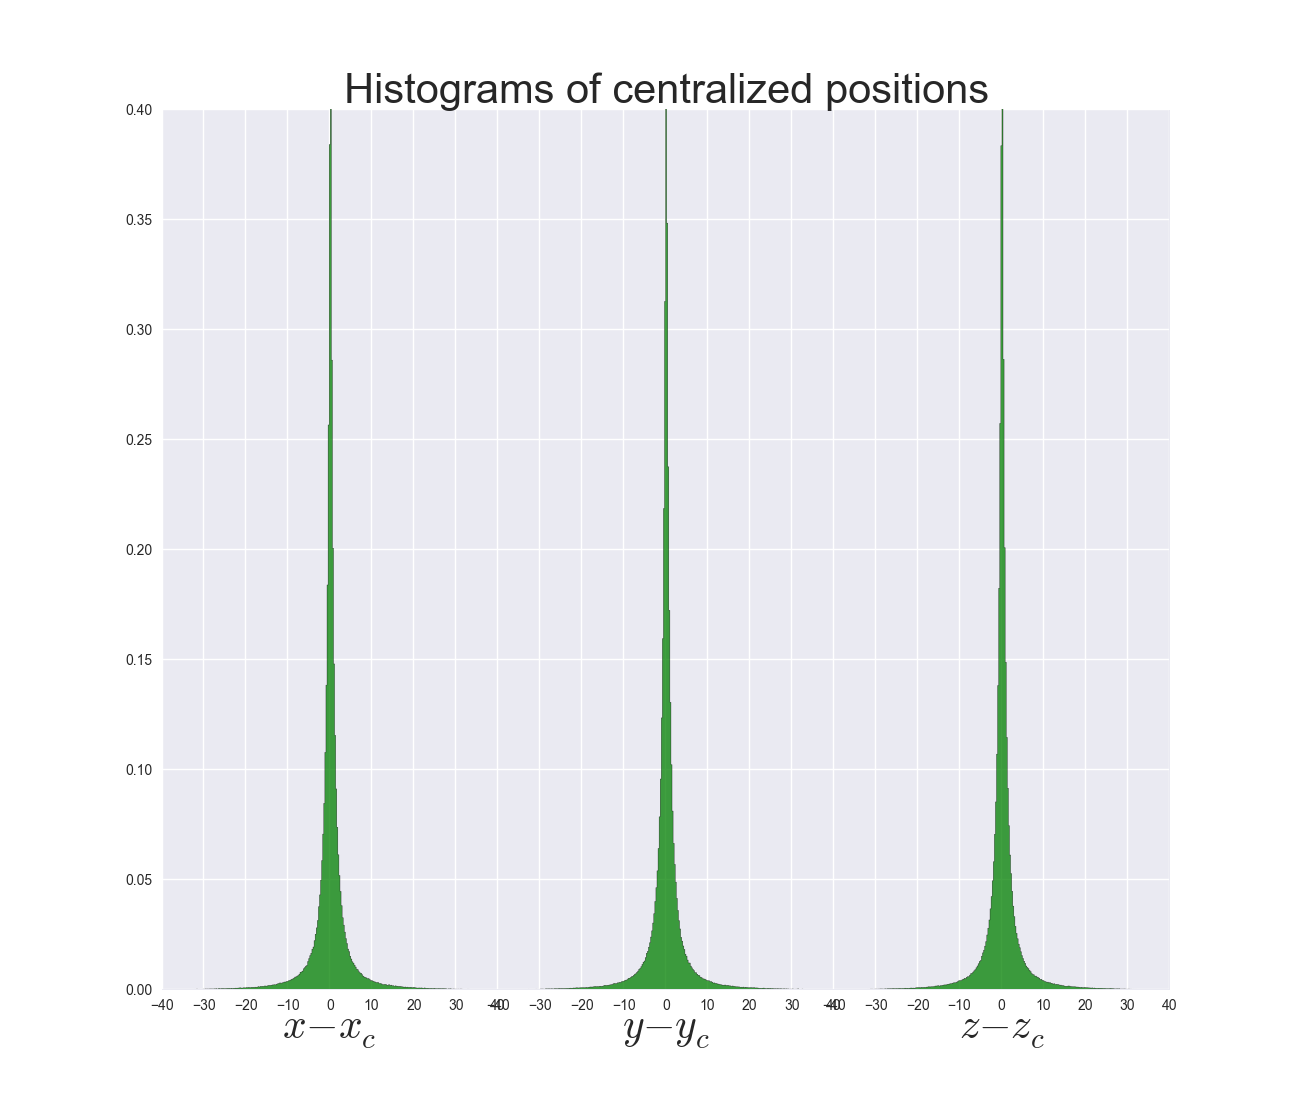
\includegraphics[width=1.0\linewidth]{img/Fig_x_hist.png}
\caption{All three cartesian coordinates are centralized around the halo center by subtraction of each individual particles position by the central coordinates $x_c$, $y_c$ and $z_c$.}
\label{fig:test}
\end{figure}

\textbf{Our Initial conditions are set up and ready to run. The next section introduces two principal ways to mimic the galaxy merger related effects. We will see how violent relaxation and phase mixing can be emulated by both sim. I and sim. II.}
